\begin{figure}
    \begin{center}
    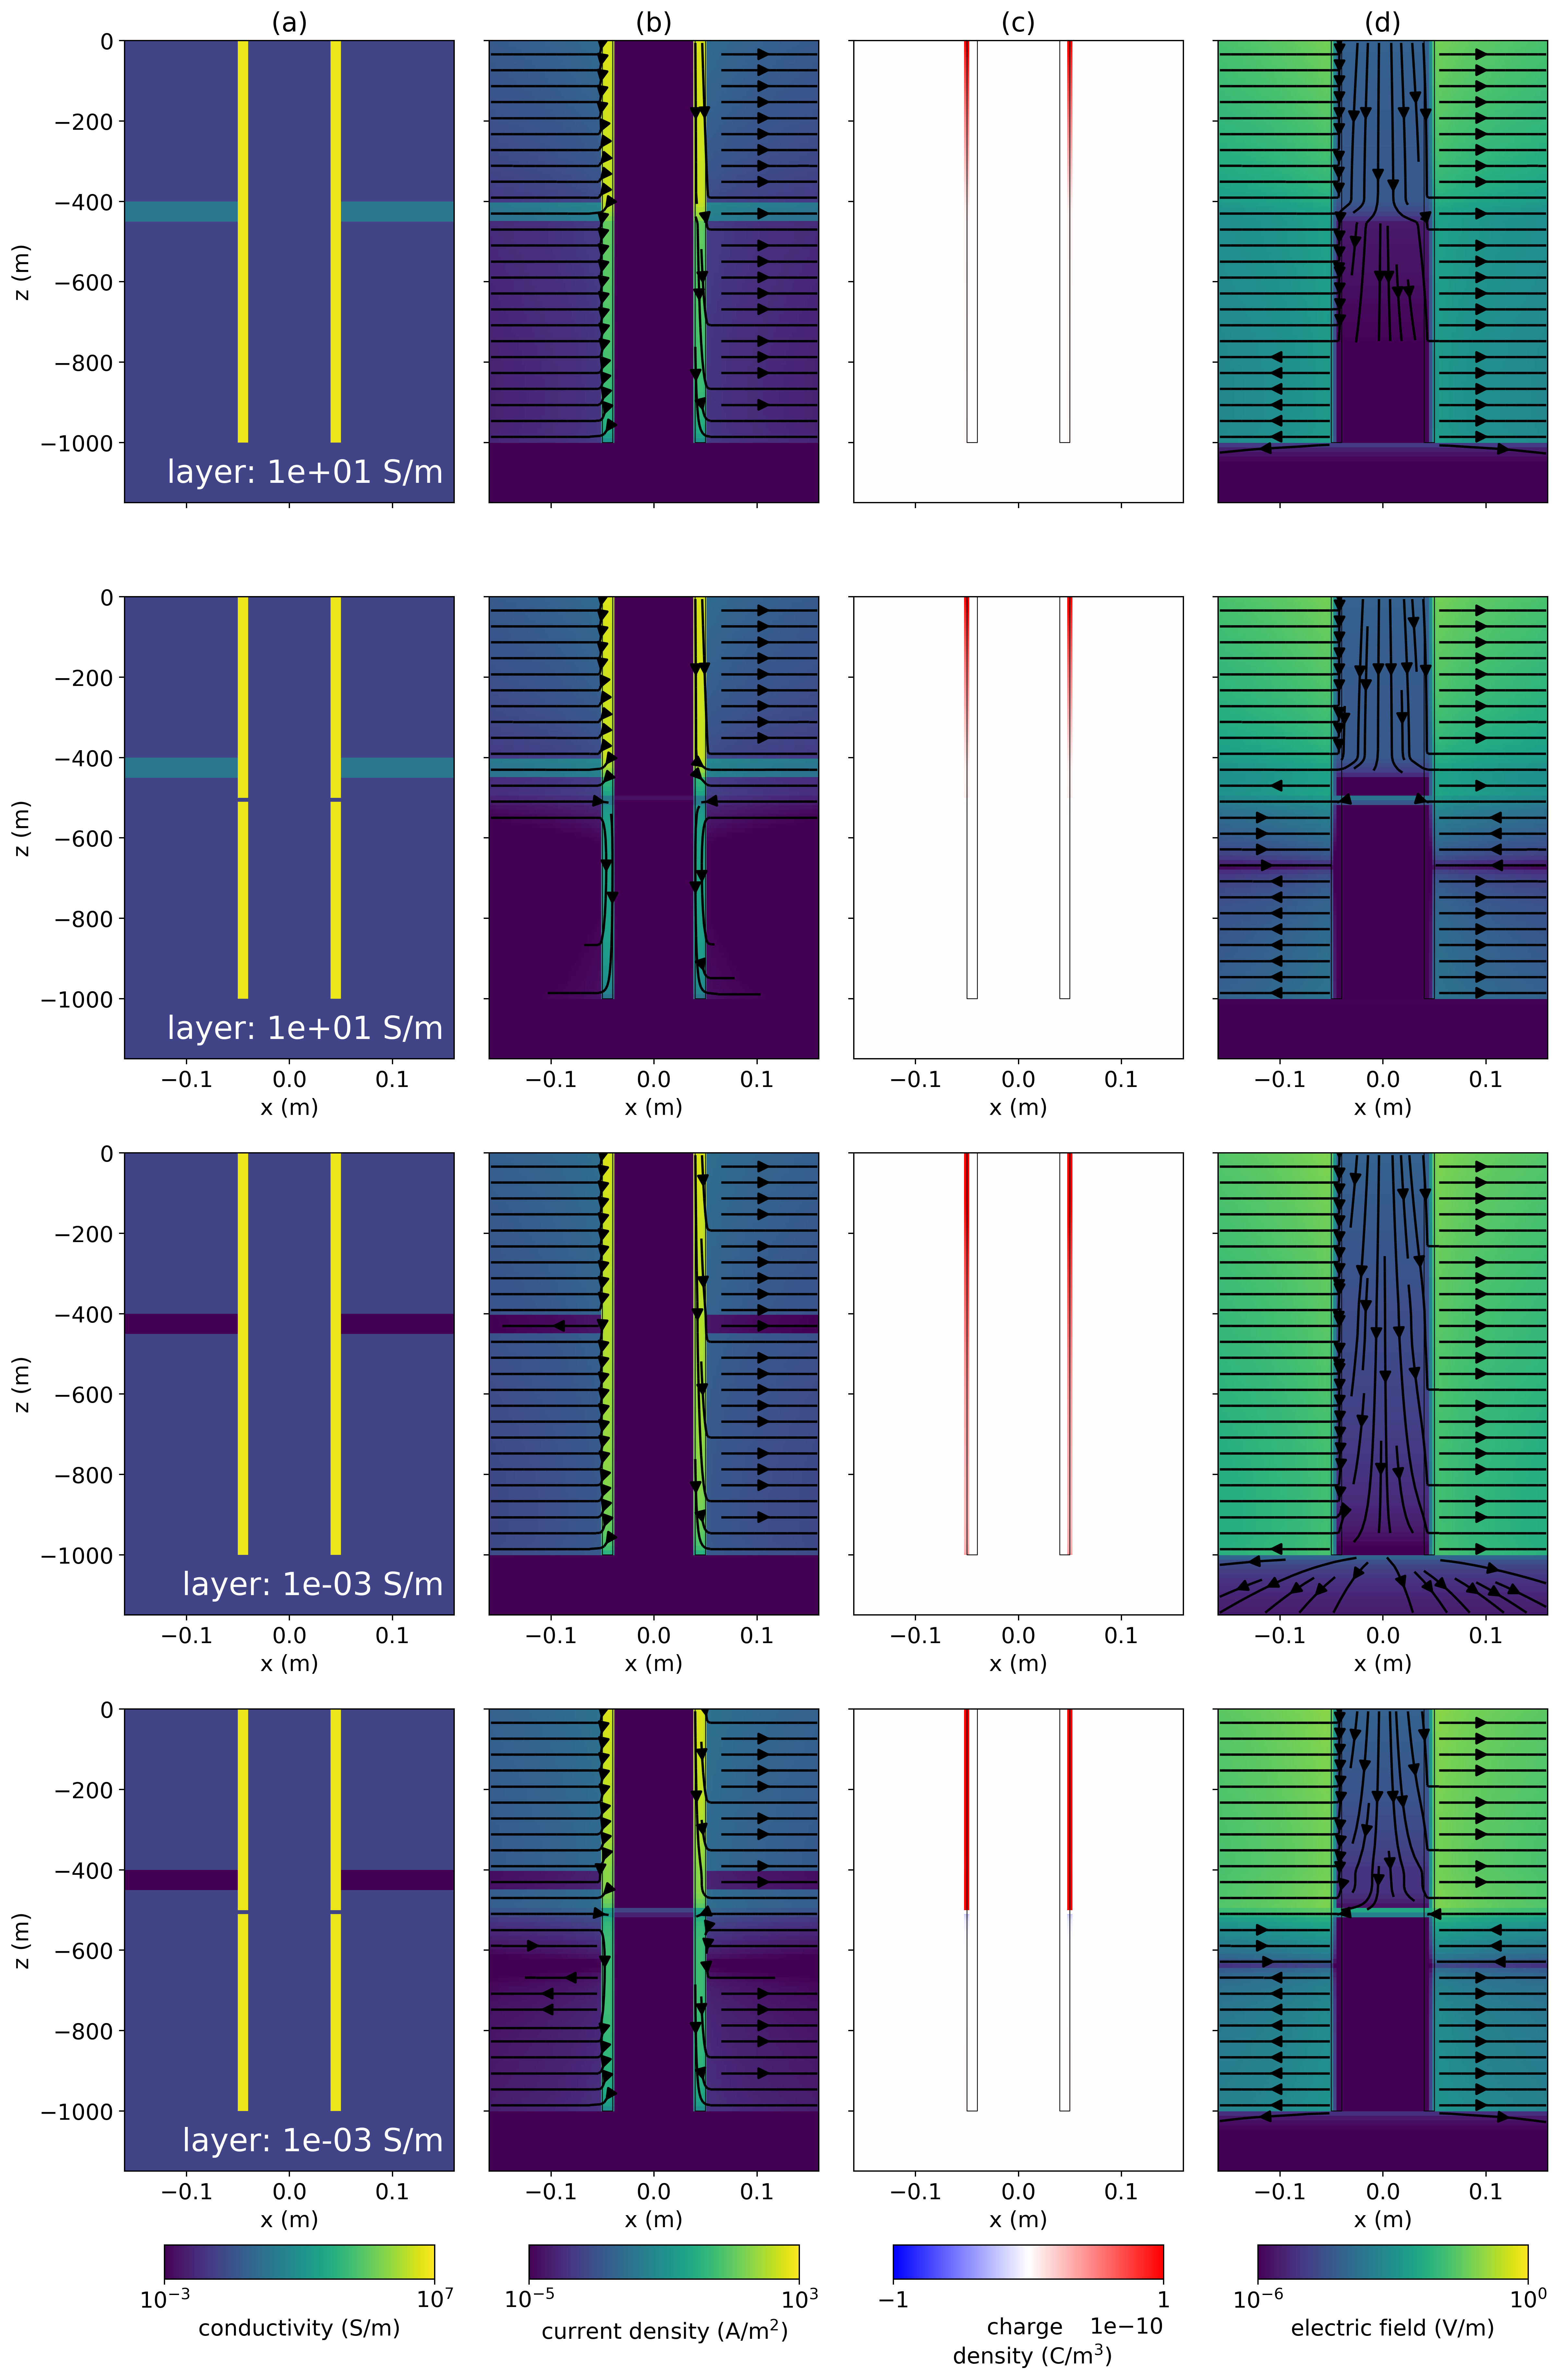
\includegraphics[width=0.8\textwidth]{figures/dc_casing/integrity_layer_physics.png}
    \end{center}
\caption{
    Cross section showing: (a) electrical conductivity, (b) current density, (c) charge density,
    and (d) electric field for a top-casing DC resistivity experiment over models with a conductive layer
    (top two rows) and a model with a resistive layer (bottom two rows). The layer extends from
    400m to 450m depth. The plots in the second and fourth correspond to models with a 10m flaw at 500m depth.
}
\label{fig:integrity_layer_physics}
\end{figure}
